\documentclass{standalone}
\usepackage{tikz}
\usetikzlibrary{patterns, positioning}
\usepackage[sfdefault]{ClearSans} %% option 'sfdefault' activates Clear Sans as the default text font
\usepackage[T1]{fontenc}

\begin{document}
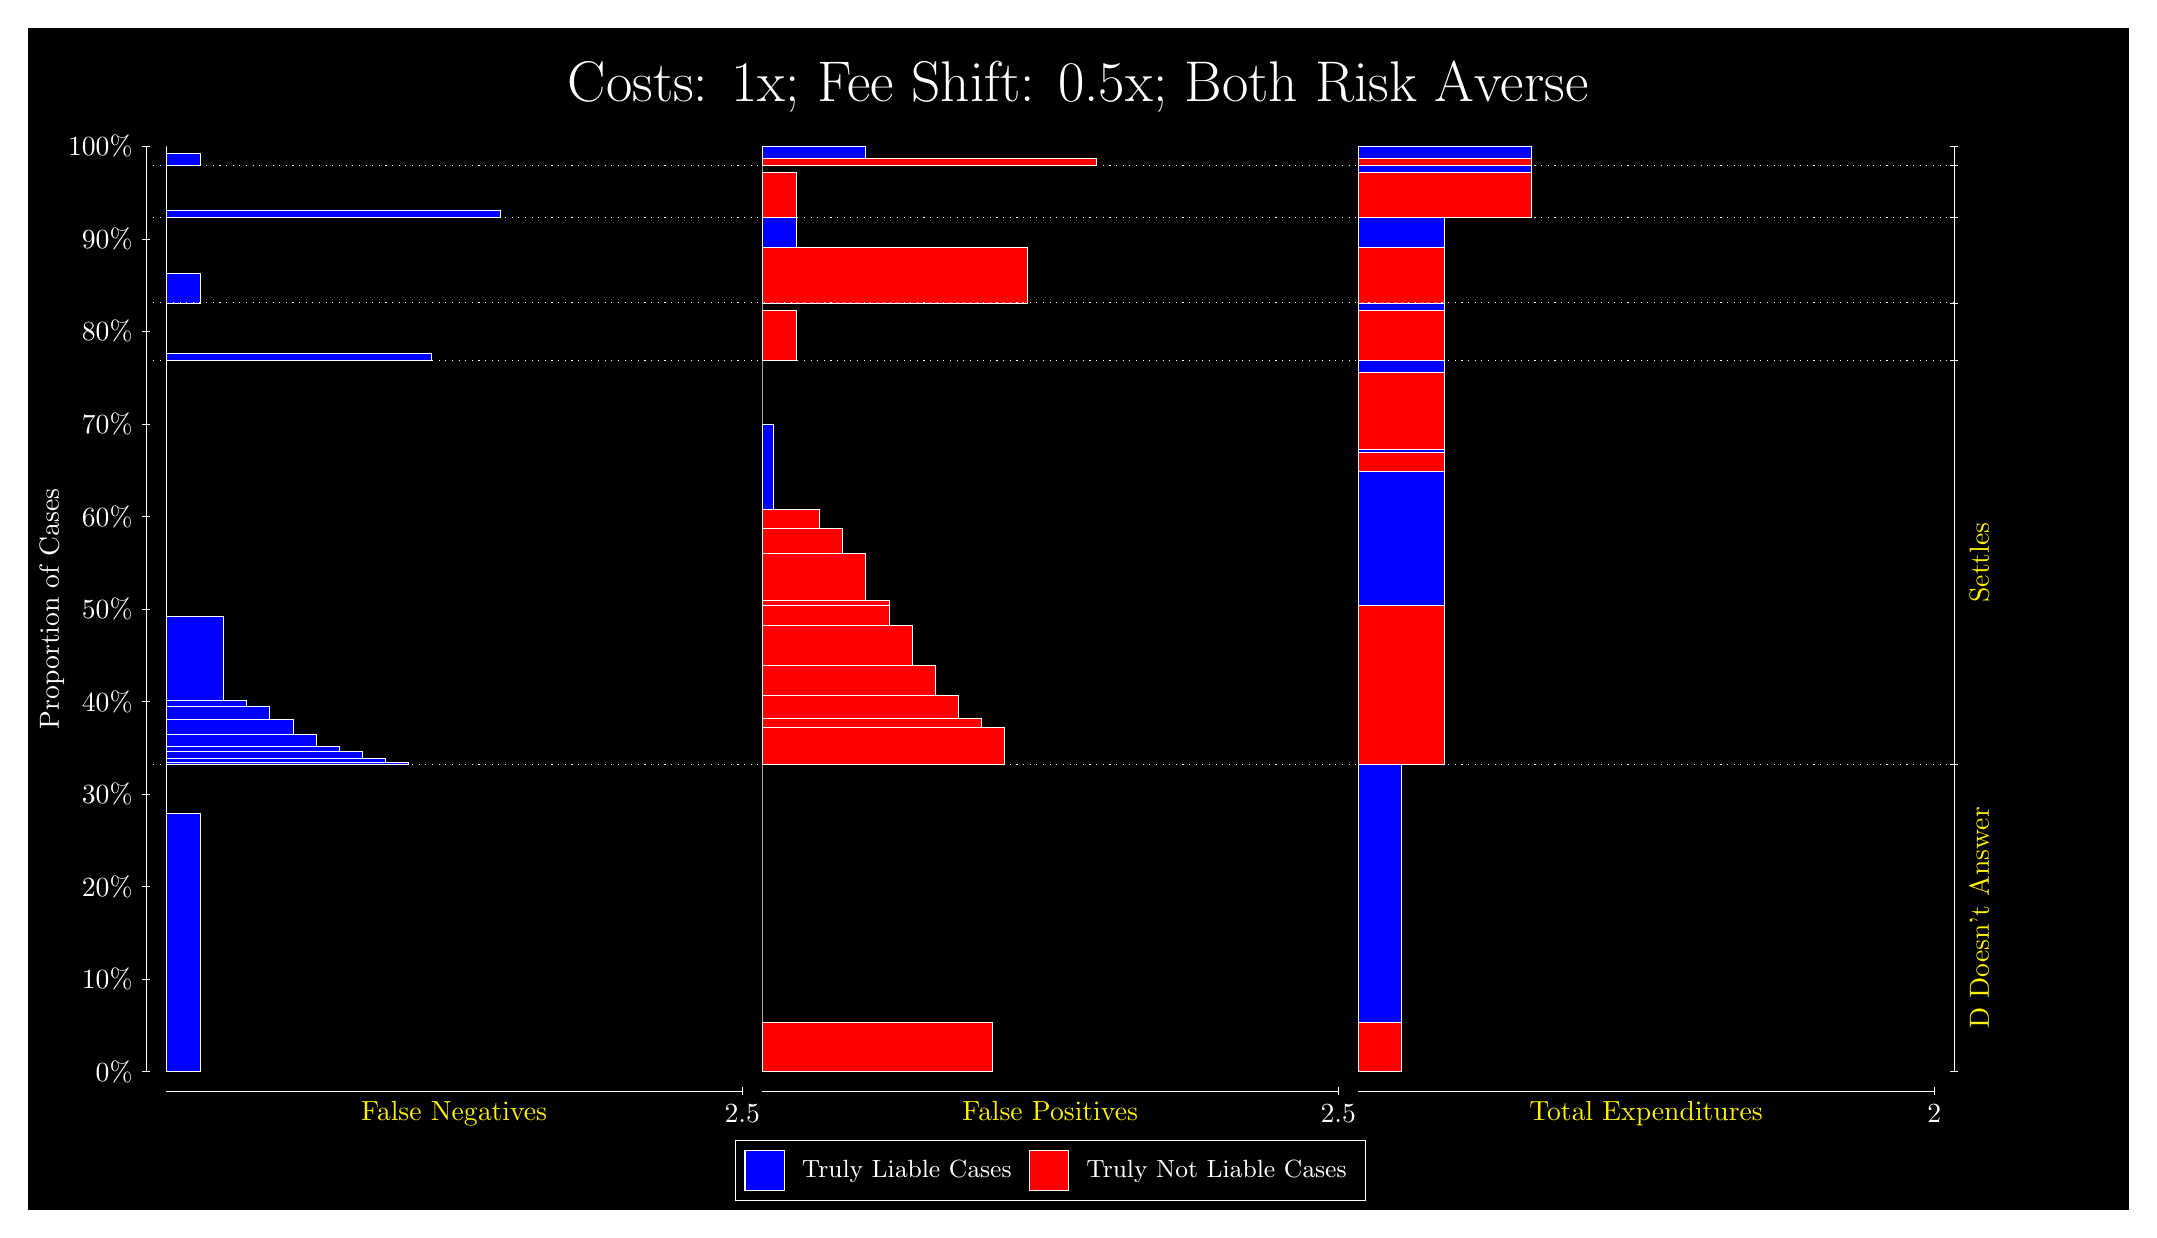
\begin{tikzpicture}
\draw[fill=black] (0,0) rectangle (26.667,15);
\draw[text=white] (0,13.5) rectangle (26.667,15) node[midway] {\huge Costs: 1x; Fee Shift: 0.5x; Both Risk Averse};
\draw[white, very thin] (1.5,1.75) -- (1.5,13.5);
\node[rotate=90, text=white, anchor=center] at (0.3, 7.625) {Proportion of Cases};
\draw[white, very thin] (1.45,1.75) -- (1.55,1.75);
\node[text=white, anchor=east] at (1.45, 1.75) {0\%};
\draw[white, very thin] (1.45,2.925) -- (1.55,2.925);
\node[text=white, anchor=east] at (1.45, 2.925) {10\%};
\draw[white, very thin] (1.45,4.1) -- (1.55,4.1);
\node[text=white, anchor=east] at (1.45, 4.1) {20\%};
\draw[white, very thin] (1.45,5.275) -- (1.55,5.275);
\node[text=white, anchor=east] at (1.45, 5.275) {30\%};
\draw[white, very thin] (1.45,6.45) -- (1.55,6.45);
\node[text=white, anchor=east] at (1.45, 6.45) {40\%};
\draw[white, very thin] (1.45,7.625) -- (1.55,7.625);
\node[text=white, anchor=east] at (1.45, 7.625) {50\%};
\draw[white, very thin] (1.45,8.8) -- (1.55,8.8);
\node[text=white, anchor=east] at (1.45, 8.8) {60\%};
\draw[white, very thin] (1.45,9.975) -- (1.55,9.975);
\node[text=white, anchor=east] at (1.45, 9.975) {70\%};
\draw[white, very thin] (1.45,11.15) -- (1.55,11.15);
\node[text=white, anchor=east] at (1.45, 11.15) {80\%};
\draw[white, very thin] (1.45,12.325) -- (1.55,12.325);
\node[text=white, anchor=east] at (1.45, 12.325) {90\%};
\draw[white, very thin] (1.45,13.5) -- (1.55,13.5);
\node[text=white, anchor=east] at (1.45, 13.5) {100\%};

\draw[white, very thin] (24.457,1.75) -- (24.457,13.5);
\draw[white, very thin] (24.407,1.75) -- (24.507,1.75);
\node[anchor=west] at (24.407, 1.75) {};
\draw[white, very thin] (24.407,5.6529) -- (24.507,5.6529);
\node[anchor=west] at (24.407, 5.6529) {};
\draw[white, very thin] (24.407,10.777) -- (24.507,10.777);
\node[anchor=west] at (24.407, 10.777) {};
\draw[white, very thin] (24.407,11.513) -- (24.507,11.513);
\node[anchor=west] at (24.407, 11.513) {};
\draw[white, very thin] (24.407,12.594) -- (24.507,12.594);
\node[anchor=west] at (24.407, 12.594) {};
\draw[white, very thin] (24.407,13.257) -- (24.507,13.257);
\node[anchor=west] at (24.407, 13.257) {};
\draw[white, very thin] (24.407,13.5) -- (24.507,13.5);
\node[anchor=west] at (24.407, 13.5) {};

\draw[white, very thin, fill=blue] (1.75,1.75) rectangle (2.1891,5.0268);
\draw[white, very thin, fill=red] (1.75,5.0268) rectangle (1.75,5.6529);
\draw[white, very thin, fill=blue] (1.75,5.6529) rectangle (4.8239,5.6834);
\draw[white, very thin, fill=blue] (1.75,5.6834) rectangle (4.5312,5.728);
\draw[white, very thin, fill=blue] (1.75,5.728) rectangle (4.2384,5.8217);
\draw[white, very thin, fill=blue] (1.75,5.8217) rectangle (3.9457,5.8786);
\draw[white, very thin, fill=blue] (1.75,5.8786) rectangle (3.6529,6.0389);
\draw[white, very thin, fill=blue] (1.75,6.0389) rectangle (3.3602,6.2254);
\draw[white, very thin, fill=blue] (1.75,6.2254) rectangle (3.0674,6.3938);
\draw[white, very thin, fill=blue] (1.75,6.3938) rectangle (2.7746,6.4662);
\draw[white, very thin, fill=blue] (1.75,6.4662) rectangle (2.4819,7.5372);
\draw[white, very thin, fill=red] (1.75,7.5372) rectangle (1.75,10.777);
\draw[white, very thin, fill=blue] (1.75,10.777) rectangle (5.1167,10.868);
\draw[white, very thin, fill=red] (1.75,10.868) rectangle (1.75,11.513);
\draw[white, very thin, fill=blue] (1.75,11.513) rectangle (2.1891,11.89);
\draw[white, very thin, fill=red] (1.75,11.89) rectangle (1.75,12.594);
\draw[white, very thin, fill=blue] (1.75,12.594) rectangle (5.9949,12.684);
\draw[white, very thin, fill=red] (1.75,12.684) rectangle (1.75,13.257);
\draw[white, very thin, fill=blue] (1.75,13.257) rectangle (2.1891,13.412);
\draw[white, very thin, fill=red] (1.75,13.412) rectangle (1.75,13.5);
\draw[white, very thin, fill=red] (9.3189,1.75) rectangle (12.246,2.3761);
\draw[white, very thin, fill=blue] (9.3189,2.3761) rectangle (9.3189,5.6529);
\draw[white, very thin, fill=red] (9.3189,5.6529) rectangle (12.393,6.1211);
\draw[white, very thin, fill=red] (9.3189,6.1211) rectangle (12.1,6.2386);
\draw[white, very thin, fill=red] (9.3189,6.2386) rectangle (11.807,6.5343);
\draw[white, very thin, fill=red] (9.3189,6.5343) rectangle (11.515,6.9069);
\draw[white, very thin, fill=red] (9.3189,6.9069) rectangle (11.222,7.4231);
\draw[white, very thin, fill=red] (9.3189,7.4231) rectangle (10.929,7.673);
\draw[white, very thin, fill=red] (9.3189,7.673) rectangle (10.929,7.7391);
\draw[white, very thin, fill=red] (9.3189,7.7391) rectangle (10.636,8.3353);
\draw[white, very thin, fill=red] (9.3189,8.3353) rectangle (10.344,8.6517);
\draw[white, very thin, fill=red] (9.3189,8.6517) rectangle (10.051,8.8927);
\draw[white, very thin, fill=blue] (9.3189,8.8927) rectangle (9.4652,9.9637);
\draw[white, very thin, fill=blue] (9.3189,9.9637) rectangle (9.3189,10.777);
\draw[white, very thin, fill=red] (9.3189,10.777) rectangle (9.758,11.421);
\draw[white, very thin, fill=blue] (9.3189,11.421) rectangle (9.3189,11.513);
\draw[white, very thin, fill=red] (9.3189,11.513) rectangle (12.686,12.217);
\draw[white, very thin, fill=blue] (9.3189,12.217) rectangle (9.758,12.594);
\draw[white, very thin, fill=red] (9.3189,12.594) rectangle (9.758,13.166);
\draw[white, very thin, fill=blue] (9.3189,13.166) rectangle (9.3189,13.257);
\draw[white, very thin, fill=red] (9.3189,13.257) rectangle (13.564,13.345);
\draw[white, very thin, fill=blue] (9.3189,13.345) rectangle (10.636,13.5);
\draw[white, very thin, fill=red] (16.888,1.75) rectangle (17.437,2.3761);
\draw[white, very thin, fill=blue] (16.888,2.3761) rectangle (17.437,5.6529);
\draw[white, very thin, fill=red] (16.888,5.6529) rectangle (17.986,7.673);
\draw[white, very thin, fill=blue] (16.888,7.673) rectangle (17.986,9.375);
\draw[white, very thin, fill=red] (16.888,9.375) rectangle (17.986,9.616);
\draw[white, very thin, fill=blue] (16.888,9.616) rectangle (17.986,9.6465);
\draw[white, very thin, fill=red] (16.888,9.6465) rectangle (17.986,10.625);
\draw[white, very thin, fill=blue] (16.888,10.625) rectangle (17.986,10.777);
\draw[white, very thin, fill=red] (16.888,10.777) rectangle (17.986,11.421);
\draw[white, very thin, fill=blue] (16.888,11.421) rectangle (17.986,11.513);
\draw[white, very thin, fill=red] (16.888,11.513) rectangle (17.986,12.217);
\draw[white, very thin, fill=blue] (16.888,12.217) rectangle (17.986,12.594);
\draw[white, very thin, fill=red] (16.888,12.594) rectangle (19.083,13.166);
\draw[white, very thin, fill=blue] (16.888,13.166) rectangle (19.083,13.257);
\draw[white, very thin, fill=red] (16.888,13.257) rectangle (19.083,13.345);
\draw[white, very thin, fill=blue] (16.888,13.345) rectangle (19.083,13.5);
\draw[white, dotted] (1.5,5.6529) -- (24.457,5.6529);
\draw[white, dotted] (1.5,10.777) -- (24.457,10.777);
\draw[white, dotted] (1.5,11.513) -- (24.457,11.513);
\draw[white, dotted] (1.5,12.594) -- (24.457,12.594);
\draw[white, dotted] (1.5,13.257) -- (24.457,13.257);
\draw[white, very thin] (1.75,1.5) -- (9.0689,1.5);
\node[text=yellow, anchor=north] at (5.4094, 1.5) {False Negatives};
\draw[white, very thin] (9.0689,1.45) -- (9.0689,1.55);
\node[text=white, anchor=north] at (9.0689, 1.45) {2.5};

\draw[white, very thin] (9.3189,1.5) -- (16.638,1.5);
\node[text=yellow, anchor=north] at (12.978, 1.5) {False Positives};
\draw[white, very thin] (16.638,1.45) -- (16.638,1.55);
\node[text=white, anchor=north] at (16.638, 1.45) {2.5};

\draw[white, very thin] (16.888,1.5) -- (24.207,1.5);
\node[text=yellow, anchor=north] at (20.547, 1.5) {Total Expenditures};
\draw[white, very thin] (24.207,1.45) -- (24.207,1.55);
\node[text=white, anchor=north] at (24.207, 1.45) {2};

\node[text=yellow, centered, rotate=90] at (24.777, 3.7014) {D Doesn't Answer};
\node[text=yellow, centered, rotate=90] at (24.777, 8.215) {Settles};





\draw (12.978300999999998,1.5) node[draw=none] (baseCoordinate) {};
\begin{scope}[align=center]
        \matrix[scale=0.5, draw=white, below=0.5cm of baseCoordinate, nodes={draw}, column sep=0.1cm]{
            \node[rectangle, draw, minimum width=0.5cm, minimum height=0.5cm, fill=blue] {}; &
            \node[draw=none, font=\small, text=white] (B) {Truly Liable Cases}; &
            \node[rectangle, draw, minimum width=0.5cm, minimum height=0.5cm, fill=red] {}; &
            \node[draw=none, font=\small, text=white] (B) {Truly Not Liable Cases}; \\
            };
\end{scope}

\end{tikzpicture}
\end{document}